%% system-matrix.tex — Per-system classification matrix
%% Included from 06-comparison.tex

\subsection{Per-System Classification}
\label{sec:system-matrix}

Table~\ref{tab:system-matrix} presents per-feature classifications for
69~systems with complete capability data across the eight discriminating
features defined in \S\ref{sec:long-tail}.  Systems are grouped by category
and sorted alphabetically within each group.

\begin{table*}[!t]
\centering
\caption{Per-system capability matrix for 69 classified systems.
$\bullet$~=~capability present.
RAG tier: N~=~Naive, A~=~Advanced, M~=~Modular~\cite{gao2023rag}.
An interactive visualization with filtering is available at
\url{https://securityronin.github.io/alaya/docs/memory-landscape.html}.}
\label{tab:system-matrix}
\scriptsize
\setlength{\tabcolsep}{3.5pt}
\begin{tabular}{@{}lc cccccccc@{}}
\toprule
\textbf{System}
  & \rotatebox{90}{\textbf{RAG}}
  & \rotatebox{90}{\textbf{Episodic}}
  & \rotatebox{90}{\textbf{Semantic}}
  & \rotatebox{90}{\textbf{Graph}}
  & \rotatebox{90}{\textbf{Fusion}}
  & \rotatebox{90}{\textbf{Consolid.}}
  & \rotatebox{90}{\textbf{Forgetting}}
  & \rotatebox{90}{\textbf{Contrad.}}
  & \rotatebox{90}{\textbf{Preference}} \\
\midrule
\multicolumn{10}{@{}l}{\textit{Dedicated Memory Systems (33)}} \\
Backboard            & A & $\bullet$ & $\bullet$ &           &           &           &           &           &           \\
ChatGPT Memory       & N & $\bullet$ &           &           &           &           & $\bullet$ &           & $\bullet$ \\
Claude Memory Tool   & N & $\bullet$ &           &           &           &           &           &           &           \\
Cognee               & A &           & $\bullet$ & $\bullet$ & $\bullet$ &           &           &           &           \\
Cortex-Mem           & N &           & $\bullet$ &           &           &           &           &           &           \\
EmergenceMem         & A & $\bullet$ & $\bullet$ &           &           &           &           &           &           \\
EverMemOS            & A & $\bullet$ & $\bullet$ &           & $\bullet$ & $\bullet$ & $\bullet$ &           &           \\
Gemini Memory        & N & $\bullet$ &           &           &           &           &           &           & $\bullet$ \\
Grok Memory          & N & $\bullet$ &           &           &           &           &           &           & $\bullet$ \\
Hindsight            & A & $\bullet$ & $\bullet$ &           & $\bullet$ &           & $\bullet$ & $\bullet$ & $\bullet$ \\
Mastra Obs.\ Mem.    & A & $\bullet$ & $\bullet$ &           &           &           &           &           &           \\
MCP Mem.\ Service    & A &           & $\bullet$ & $\bullet$ & $\bullet$ &           &           &           &           \\
Mem0                 & A & $\bullet$ & $\bullet$ & $\bullet$ & $\bullet$ &           & $\bullet$ & $\bullet$ & $\bullet$ \\
Memary               & A &           & $\bullet$ & $\bullet$ &           &           & $\bullet$ &           &           \\
MemMachine           & A & $\bullet$ & $\bullet$ &           &           &           &           &           &           \\
Memobase             & N &           &           &           &           &           &           &           & $\bullet$ \\
MemOS                & A & $\bullet$ & $\bullet$ & $\bullet$ & $\bullet$ & $\bullet$ & $\bullet$ &           & $\bullet$ \\
MemoryOS             & A & $\bullet$ & $\bullet$ &           & $\bullet$ &           & $\bullet$ &           & $\bullet$ \\
Memonto              & N &           & $\bullet$ & $\bullet$ &           &           &           &           &           \\
Memvid               & A & $\bullet$ &           &           & $\bullet$ &           &           &           &           \\
Meta AI Memory       & N & $\bullet$ &           &           &           &           &           &           &           \\
Motorhead            & N & $\bullet$ &           &           &           &           & $\bullet$ &           &           \\
Neo4j Agent Mem.     & A & $\bullet$ & $\bullet$ & $\bullet$ & $\bullet$ &           &           &           &           \\
OpenClaw Redis       & A & $\bullet$ & $\bullet$ &           &           &           & $\bullet$ &           & $\bullet$ \\
OpenMemory           & A & $\bullet$ & $\bullet$ & $\bullet$ & $\bullet$ &           & $\bullet$ &           & $\bullet$ \\
OpenViking           & N & $\bullet$ &           &           &           &           &           &           &           \\
Papr Memory          & A & $\bullet$ & $\bullet$ &           &           &           &           &           &           \\
Perplexity Memory    & A & $\bullet$ &           &           &           &           &           &           & $\bullet$ \\
Redis Memory         & A &           & $\bullet$ &           & $\bullet$ &           &           &           &           \\
Supermemory          & A & $\bullet$ & $\bullet$ & $\bullet$ &           &           & $\bullet$ &           & $\bullet$ \\
TiMem                & A & $\bullet$ & $\bullet$ &           &           & $\bullet$ & $\bullet$ &           &           \\
Vestige              & M & $\bullet$ & $\bullet$ & $\bullet$ & $\bullet$ &           & $\bullet$ &           & $\bullet$ \\
Zep/Graphiti         & M & $\bullet$ & $\bullet$ & $\bullet$ & $\bullet$ & $\bullet$ & $\bullet$ & $\bullet$ &           \\
\midrule
\multicolumn{10}{@{}l}{\textit{Framework Memory Modules (10)}} \\
Agency Swarm         & N & $\bullet$ &           &           &           &           &           &           &           \\
AutoGPT              & N & $\bullet$ &           &           &           &           &           &           &           \\
CrewAI               & A & $\bullet$ & $\bullet$ &           & $\bullet$ &           &           &           & $\bullet$ \\
Haystack             & N & $\bullet$ &           &           &           &           &           &           &           \\
LangChain            & N & $\bullet$ &           &           &           &           & $\bullet$ &           &           \\
LangMem SDK          & N &           & $\bullet$ &           &           &           &           &           &           \\
Letta (MemGPT)       & N & $\bullet$ & $\bullet$ &           &           & $\bullet$ & $\bullet$ &           & $\bullet$ \\
LlamaIndex           & N & $\bullet$ &           &           &           &           & $\bullet$ &           &           \\
MS GraphRAG          & M &           & $\bullet$ & $\bullet$ & $\bullet$ &           &           &           &           \\
Qwen-Agent           & N & $\bullet$ &           &           &           &           &           &           &           \\
\midrule
\multicolumn{10}{@{}l}{\textit{Coding Agent Memory (9)}} \\
Basic Memory         & A &           & $\bullet$ & $\bullet$ &           &           &           &           &           \\
Beads                & A & $\bullet$ & $\bullet$ & $\bullet$ &           & $\bullet$ & $\bullet$ &           &           \\
Cipher (ByteRover)   & A & $\bullet$ & $\bullet$ &           &           &           & $\bullet$ &           &           \\
Clawdbot-Next        & A & $\bullet$ &           &           & $\bullet$ &           &           &           &           \\
ClaudeHistory Cloud  & N & $\bullet$ &           &           &           &           &           &           &           \\
Engram               & N & $\bullet$ &           &           &           &           &           &           &           \\
MemoryMesh           & N & $\bullet$ &           &           &           &           &           &           &           \\
Memsearch            & A & $\bullet$ &           &           &           &           & $\bullet$ &           &           \\
QMD                  & M & $\bullet$ & $\bullet$ &           & $\bullet$ &           &           &           &           \\
\midrule
\multicolumn{10}{@{}l}{\textit{File-Based Memory (2)}} \\
Claude Code          & N & $\bullet$ &           &           &           &           &           &           & $\bullet$ \\
Claudesidian         & A & $\bullet$ &           & $\bullet$ &           &           & $\bullet$ &           &           \\
\midrule
\multicolumn{10}{@{}l}{\textit{Research Architectures (15)}} \\
A-MEM                & A &           & $\bullet$ & $\bullet$ & $\bullet$ &           &           &           &           \\
AgeMem               & A & $\bullet$ &           &           &           &           & $\bullet$ &           &           \\
G-Memory             & A & $\bullet$ & $\bullet$ &           &           &           &           & $\bullet$ &           \\
Generative Agents    & A & $\bullet$ & $\bullet$ &           & $\bullet$ & $\bullet$ & $\bullet$ &           & $\bullet$ \\
HippoRAG             & M &           & $\bullet$ & $\bullet$ &           &           &           &           &           \\
HippoRAG~2           & M & $\bullet$ & $\bullet$ & $\bullet$ & $\bullet$ &           &           &           &           \\
LightMem             & A & $\bullet$ & $\bullet$ &           &           & $\bullet$ & $\bullet$ &           &           \\
LightRAG             & M &           & $\bullet$ & $\bullet$ & $\bullet$ &           &           &           &           \\
Mem-alpha            & A & $\bullet$ & $\bullet$ &           &           &           & $\bullet$ &           &           \\
MemAgent             & A & $\bullet$ &           &           &           &           & $\bullet$ &           &           \\
MemoryBank           & A & $\bullet$ & $\bullet$ &           &           &           & $\bullet$ &           & $\bullet$ \\
MemoRAG              & A & $\bullet$ & $\bullet$ &           & $\bullet$ &           &           &           &           \\
MemRL                & A & $\bullet$ &           &           &           &           & $\bullet$ &           &           \\
Memory-R1            & A & $\bullet$ &           &           &           &           & $\bullet$ &           &           \\
SYNAPSE              & M & $\bullet$ & $\bullet$ & $\bullet$ & $\bullet$ & $\bullet$ & $\bullet$ &           &           \\
\bottomrule
\end{tabular}
\end{table*}

Three patterns emerge from the per-system view that are not visible in the
aggregate statistics.  First, contradiction resolution is the rarest
capability: only 4 of 69~systems implement it (Mem0, Zep/Graphiti,
Hindsight, and G-Memory), spanning dedicated and research categories.
Second, Modular RAG systems implement more lifecycle operations
(consolidation, forgetting) than Naive or Advanced RAG systems---retrieval
sophistication correlates with architectural investment in lifecycle
operations.  Third, framework memory modules implement at most five of the
eight features: memory is a secondary concern in orchestration frameworks,
limiting investment in consolidation, contradiction resolution, and
graph-based retrieval.

\begin{figure}[!t]
\centering
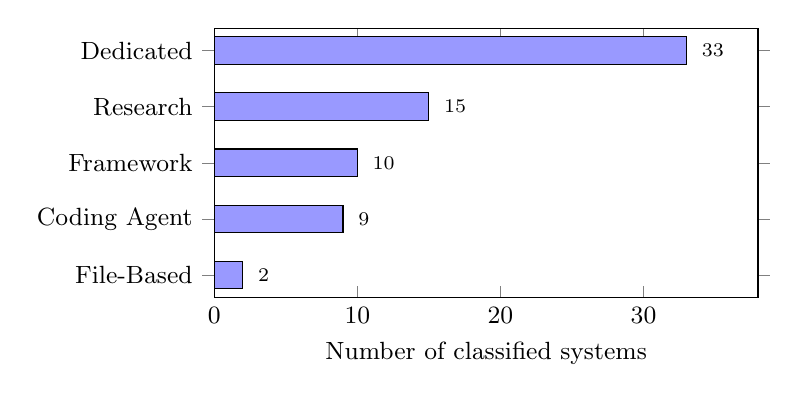
\begin{tikzpicture}
\begin{axis}[
    xbar,
    width=0.7\columnwidth,
    height=5cm,
    xlabel={Number of classified systems},
    symbolic y coords={File-Based, Coding Agent, Framework, Research, Dedicated},
    ytick=data,
    xmin=0, xmax=38,
    nodes near coords,
    nodes near coords style={font=\scriptsize, anchor=west},
    every node near coord/.append style={xshift=2pt},
    bar width=10pt,
    x tick label style={font=\small},
    y tick label style={font=\small},
    xlabel style={font=\small},
]
\addplot[fill=blue!40] coordinates {
    (2,File-Based)
    (9,Coding Agent)
    (10,Framework)
    (15,Research)
    (33,Dedicated)
};
\end{axis}
\end{tikzpicture}
\caption{Number of classified systems by category.  Dedicated memory systems
dominate the landscape, reflecting the field's focus on memory as a primary
architectural concern.  Framework modules and coding agent tools are
underrepresented, consistent with memory being an auxiliary feature in
these categories.}
\label{fig:category-scores}
\end{figure}

Figure~\ref{fig:category-scores} summarizes the category-level pattern:
dedicated systems dominate the classified landscape, while framework modules
and coding tools remain underrepresented---consistent with memory being a
secondary concern in orchestration and development tool contexts.

Figure~\ref{fig:quadrant} plots each system along two orthogonal dimensions
derived from the capability matrix: \emph{structure breadth} (count of
episodic, semantic, graph, and fusion capabilities; $x$-axis) and
\emph{lifecycle depth} (count of consolidation, forgetting, contradiction
resolution, and preference learning; $y$-axis).  The resulting quadrant
reveals the field's central tension: the bottom-right quadrant
(retrieval-focused, lifecycle-sparse) is densely populated, while the
top-right (full-stack memory) contains only a handful of systems.
No system achieves the maximum on both axes simultaneously.

\begin{figure*}[!t]
\centering
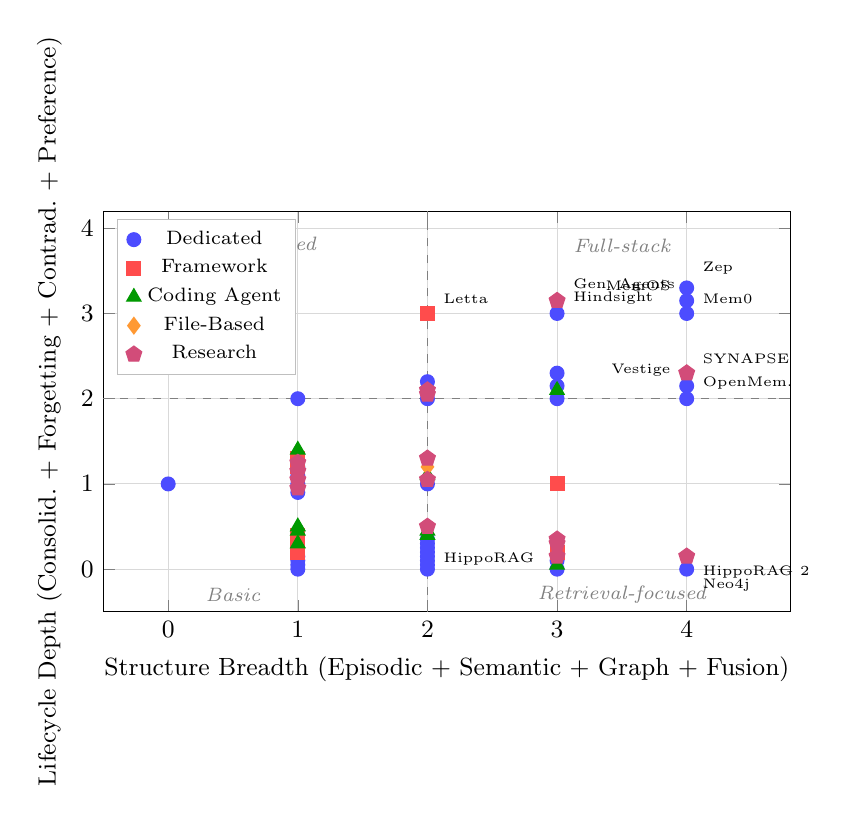
\begin{tikzpicture}
\begin{axis}[
    width=0.85\textwidth,
    height=0.55\textwidth,
    xlabel={Structure Breadth (Episodic + Semantic + Graph + Fusion)},
    ylabel={Lifecycle Depth (Consolid.\ + Forgetting + Contrad.\ + Preference)},
    xmin=-0.5, xmax=4.8,
    ymin=-0.5, ymax=4.2,
    xtick={0,1,2,3,4},
    ytick={0,1,2,3,4},
    grid=major,
    grid style={gray!30},
    xlabel style={font=\small},
    ylabel style={font=\small},
    tick label style={font=\small},
    legend style={font=\scriptsize, at={(0.02,0.98)}, anchor=north west, draw=gray!50},
    clip=false,
]
% Quadrant labels
\node[font=\scriptsize\itshape, gray] at (axis cs:0.5,3.8) {Lifecycle-focused};
\node[font=\scriptsize\itshape, gray] at (axis cs:3.5,3.8) {Full-stack};
\node[font=\scriptsize\itshape, gray] at (axis cs:0.5,-0.3) {Basic};
\node[font=\scriptsize\itshape, gray] at (axis cs:3.5,-0.3) {Retrieval-focused};
% Quadrant dividers
\draw[gray, dashed] (axis cs:2,-0.5) -- (axis cs:2,4.2);
\draw[gray, dashed] (axis cs:-0.5,2) -- (axis cs:4.8,2);

% --- Dedicated Memory Systems (filled circles) ---
\addplot[only marks, mark=*, blue!70, mark size=2.5pt] coordinates {
    (2,0)      % Backboard
    (1,2)      % ChatGPT Memory
    (1,0)      % Claude Memory Tool
    (3,0)      % Cognee
    (1,0.05)   % Cortex-Mem (jitter)
    (2,0.1)    % EmergenceMem (jitter)
    (3,2)      % EverMemOS
    (1,1)      % Gemini Memory
    (1,1.1)    % Grok Memory (jitter)
    (3,3)      % Hindsight
    (2,0.2)    % Mastra (jitter)
    (3,0.1)    % MCP Mem Service (jitter)
    (4,3)      % Mem0
    (2,1)      % Memary
    (2,0.3)    % MemMachine (jitter)
    (0,1)      % Memobase
    (4,3.15)   % MemOS (jitter)
    (3,2.15)   % MemoryOS (jitter)
    (2,0.05)   % Memonto (jitter)
    (2,0.15)   % Memvid (jitter)
    (1,0.1)    % Meta AI Memory (jitter)
    (1,1.2)    % Motorhead (jitter)
    (4,0)      % Neo4j Agent Mem
    (2,2)      % OpenClaw Redis
    (4,2)      % OpenMemory
    (1,0.15)   % OpenViking (jitter)
    (2,0.35)   % Papr (jitter)
    (1,0.9)    % Perplexity Memory (jitter)
    (2,0.25)   % Redis Memory (jitter)
    (3,2.3)    % Supermemory (jitter)
    (2,2.2)    % TiMem (jitter)
    (4,2.15)   % Vestige (jitter)
    (4,3.3)    % Zep/Graphiti (jitter)
};

% --- Framework Memory Modules (squares) ---
\addplot[only marks, mark=square*, red!70, mark size=2.5pt] coordinates {
    (1,0.2)    % Agency Swarm (jitter)
    (1,0.25)   % AutoGPT (jitter)
    (3,1)      % CrewAI
    (1,0.3)    % Haystack (jitter)
    (1,1.2)    % LangChain (jitter)
    (1,0.35)   % LangMem SDK (jitter)
    (2,3)      % Letta (MemGPT)
    (1,1.3)    % LlamaIndex (jitter)
    (3,0.2)    % MS GraphRAG (jitter)
    (1,0.4)    % Qwen-Agent (jitter)
};

% --- Coding Agent Memory (triangles) ---
\addplot[only marks, mark=triangle*, green!60!black, mark size=3pt] coordinates {
    (2,0.4)    % Basic Memory (jitter)
    (3,2.1)    % Beads (jitter)
    (2,1.1)    % Cipher (jitter)
    (2,0.45)   % Clawdbot-Next (jitter)
    (1,0.45)   % ClaudeHistory Cloud (jitter)
    (1,0.3)    % Engram (jitter)
    (1,0.5)    % MemoryMesh (jitter)
    (1,1.4)    % Memsearch (jitter)
    (3,0.05)   % QMD (jitter)
};

% --- File-Based Memory (diamonds) ---
\addplot[only marks, mark=diamond*, orange!80, mark size=3pt] coordinates {
    (1,1.15)   % Claude Code (jitter)
    (2,1.2)    % Claudesidian (jitter)
};

% --- Research Architectures (pentagons/stars) ---
\addplot[only marks, mark=pentagon*, purple!70, mark size=3pt] coordinates {
    (3,0.3)    % A-MEM (jitter)
    (1,0.95)   % AgeMem (jitter)
    (2,1.05)   % G-Memory (jitter)
    (3,3.15)   % Generative Agents (jitter)
    (2,0.5)    % HippoRAG (jitter)
    (4,0.15)   % HippoRAG 2 (jitter)
    (2,2.1)    % LightMem (jitter)
    (3,0.15)   % LightRAG (jitter)
    (2,1.3)    % Mem-alpha (jitter)
    (1,1.05)   % MemAgent (jitter)
    (2,2.05)   % MemoryBank (jitter)
    (3,0.35)   % MemoRAG (jitter)
    (1,1.15)   % MemRL (jitter)
    (1,1.25)   % Memory-R1 (jitter)
    (4,2.3)    % SYNAPSE (jitter)
};

\legend{Dedicated, Framework, Coding Agent, File-Based, Research}

% Labels for notable systems
\node[font=\tiny, anchor=south west] at (axis cs:4.05,3.35) {Zep};
\node[font=\tiny, anchor=south west] at (axis cs:4.05,3) {Mem0};
\node[font=\tiny, anchor=south east] at (axis cs:3.95,3.15) {MemOS};
\node[font=\tiny, anchor=south west] at (axis cs:3.05,3) {Hindsight};
\node[font=\tiny, anchor=south west] at (axis cs:3.05,3.15) {Gen.\ Agents};
\node[font=\tiny, anchor=south west] at (axis cs:2.05,3) {Letta};
\node[font=\tiny, anchor=south west] at (axis cs:4.05,2.3) {SYNAPSE};
\node[font=\tiny, anchor=south west] at (axis cs:4.05,2) {OpenMem.};
\node[font=\tiny, anchor=south east] at (axis cs:3.95,2.15) {Vestige};
\node[font=\tiny, anchor=north west] at (axis cs:4.05,0.15) {HippoRAG~2};
\node[font=\tiny, anchor=north west] at (axis cs:4.05,0) {Neo4j};
\node[font=\tiny, anchor=north west] at (axis cs:2.05,0.3) {HippoRAG};
\end{axis}
\end{tikzpicture}
\caption{Memory system quadrant.  Each system is plotted by its
\emph{structure breadth} (number of storage and retrieval capabilities) vs.\
\emph{lifecycle depth} (number of memory evolution operations).  The
bottom-right quadrant (retrieval-focused, lifecycle-sparse) is densely
populated; the top-right (full-stack) contains only a few systems.
Marker shapes distinguish system categories.}
\label{fig:quadrant}
\end{figure*}

Table~\ref{tab:rag-breadth} cross-tabulates RAG tier with mean feature
breadth count.  The progression is monotonic: Naive RAG systems average
1.6 features, Advanced 3.4, and Modular 4.3---confirming that retrieval
sophistication is a reliable proxy for overall architectural investment
in memory lifecycle operations.

\begin{table}[!t]
\centering
\caption{Mean feature breadth by RAG tier for 69 classified systems.
Feature count tallies the same eight capabilities as
Table~\ref{tab:capability-distribution}.}
\label{tab:rag-breadth}
\small
\begin{tabular}{@{}lrrrr@{}}
\toprule
\textbf{RAG Tier} & \textbf{$N$} & \textbf{Mean} & \textbf{Min} & \textbf{Max} \\
\midrule
Naive    & 22 & 1.6 & 1 & 5 \\
Advanced & 39 & 3.4 & 2 & 7 \\
Modular  &  8 & 4.3 & 2 & 7 \\
\bottomrule
\end{tabular}
\end{table}

Table~\ref{tab:cooccurrence} reveals pairwise feature co-occurrence
across the 69 classified systems.  Two correlations are striking.
First, consolidation and forgetting are perfectly co-occurrent: all 9
systems with consolidation also implement forgetting, consistent with
the architectural argument that consolidation creates a growing semantic
store that requires active management.  Second, graph structure and
fusion are strongly correlated (13 of 20 graph systems also use fusion),
confirming that graph traversal provides a third retrieval signal that
motivates principled fusion.  Contradiction resolution is the most
isolated feature: only 4 systems implement it, all of which also have
both episodic and semantic storage---suggesting it requires a mature
architectural foundation.

\begin{table}[!t]
\centering
\caption{Feature co-occurrence matrix (lower triangle) for 69 classified
systems.  Diagonal (bold) shows total count per feature.  Notable:
Consolidation $\leftrightarrow$ Forgetting = 9/9 (100\%);
Graph $\leftrightarrow$ Fusion = 13/20 (65\%).}
\label{tab:cooccurrence}
\scriptsize
\setlength{\tabcolsep}{3pt}
\begin{tabular}{@{}lrrrrrrrr@{}}
\toprule
& \rotatebox{70}{\textbf{Ep.}}
& \rotatebox{70}{\textbf{Sem.}}
& \rotatebox{70}{\textbf{Graph}}
& \rotatebox{70}{\textbf{Fusion}}
& \rotatebox{70}{\textbf{Consol.}}
& \rotatebox{70}{\textbf{Forget.}}
& \rotatebox{70}{\textbf{Contrad.}}
& \rotatebox{70}{\textbf{Pref.}} \\
\midrule
Episodic      & \textbf{56} \\
Semantic      & 30 & \textbf{42} \\
Graph         & 11 & 19 & \textbf{20} \\
Fusion        & 17 & 21 & 13 & \textbf{23} \\
Consolidation &  9 &  9 &  4 &  5 & \textbf{9} \\
Forgetting    & 29 & 20 & 10 & 10 &  9 & \textbf{30} \\
Contradiction &  4 &  4 &  2 &  3 &  1 &  3 & \textbf{4} \\
Preference    & 17 & 12 &  5 &  8 &  3 & 12 &  2 & \textbf{18} \\
\bottomrule
\end{tabular}
\end{table}

Figure~\ref{fig:decision-tree} provides a practitioner-facing decision
tree for selecting a memory architecture based on deployment requirements.
The tree routes through three questions---memory volume, associative
retrieval needs, and lifecycle requirements---to arrive at representative
systems for each configuration.

\begin{figure*}[!t]
\centering
\begin{tikzpicture}[
    decision/.style={diamond, draw, fill=blue!8, text width=2.2cm,
                     align=center, inner sep=1pt, font=\scriptsize},
    result/.style={rectangle, draw, rounded corners, fill=green!10,
                   text width=2.6cm, align=center, font=\scriptsize,
                   minimum height=0.8cm},
    arr/.style={->, >=Stealth, thick},
    lab/.style={font=\tiny, fill=white, inner sep=1pt},
]
% Level 0
\node[decision] (q1) at (0,0) {Memory\\$>$100K tokens?};
% Level 1 - No
\node[result] (r0) at (-5,-2) {Windowed context\\LangChain, LlamaIndex,\\Letta};
% Level 1 - Yes
\node[decision] (q2) at (3,-2) {Need graph/\\relational\\queries?};
% Level 2 - Yes
\node[decision] (q3) at (0,-4.5) {Need lifecycle\\(forget, consol.)?};
% Level 2 - No
\node[decision] (q4) at (6,-4.5) {Need user\\personalization?};
% Level 3
\node[result] (r1) at (-2,-6.8) {Full-stack\\Zep, SYNAPSE,\\MemOS, Mem0};
\node[result] (r2) at (2,-6.8) {Graph retrieval\\HippoRAG~2, LightRAG,\\Cognee, Neo4j};
\node[result] (r3) at (4.5,-6.8) {Preference\\Hindsight, ChatGPT\\Mem., OpenMemory};
\node[result] (r4) at (7.5,-6.8) {Standard RAG\\Engram, Memvid,\\basic vector store};
% Edges
\draw[arr] (q1) -| node[lab,above left] {no} (r0);
\draw[arr] (q1) -- node[lab,right] {yes} (q2);
\draw[arr] (q2) -- node[lab,left] {yes} (q3);
\draw[arr] (q2) -- node[lab,right] {no} (q4);
\draw[arr] (q3) -- node[lab,left] {yes} (r1);
\draw[arr] (q3) -- node[lab,right] {no} (r2);
\draw[arr] (q4) -- node[lab,left] {yes} (r3);
\draw[arr] (q4) -- node[lab,right] {no} (r4);
\end{tikzpicture}
\caption{Practitioner decision tree for selecting a memory architecture.
Each decision node corresponds to a deployment requirement; leaf nodes
list representative systems.  The tree reflects the feature clustering
in \S\ref{sec:long-tail}: graph traversal and lifecycle operations
partition the landscape into distinct architectural tiers.}
\label{fig:decision-tree}
\end{figure*}

For interactive exploration with filtering by category, capability, RAG
tier, and lifecycle operations, see the companion
visualization.\footnote{\url{https://securityronin.github.io/alaya/docs/memory-landscape.html}
The visualization includes the full 69-system matrix with sortable
columns, the quadrant plot with hover details, and the co-occurrence
heatmap with color encoding.}
